\documentclass[journal]{IEEEtran}
\usepackage{amsmath}
\usepackage{amssymb}
\usepackage{booktabs}
\usepackage{cite}
\usepackage{listings}
\usepackage{tikz}
\usepackage{url}
\usepackage{xcolor}
\usepackage{microtype}
\usetikzlibrary{arrows.meta, positioning, fit}

\definecolor{codeblue}{RGB}{0,45,115}
\definecolor{codegray}{RGB}{90,90,90}
\definecolor{codegreen}{RGB}{0,100,0}
\definecolor{codebackground}{RGB}{247,249,252}
\definecolor{codeborder}{RGB}{180,190,205}
\lstdefinelanguage{Zig}{
  sensitive=true,
  morekeywords={addrspace,align,allowzero,anyframe,anytype,asm,async,await,
    break,catch,comptime,const,continue,defer,else,enum,errdefer,error,
    export,extern,false,fn,for,noalias,noinline,nosuspend,opaque,or,
    orelse,packed,pub,return,struct,suspend,switch, test,threadlocal,
    true,try,undefined,union,unreachable,usingnamespace,var,volatile,while,
    u8,u16,u32,u64,u128,i8,i16,i32,i64,i128,usize,isize,f32,f64,bool,void},
  morecomment=[l]{//},
  morecomment=[s]{/*}{*/},
  morestring=[b]"
}
\lstset{
  basicstyle=\footnotesize\ttfamily,
  keywordstyle=\color{codeblue},
  commentstyle=\color{codegreen},
  stringstyle=\color{codegray},
  numbers=left,
  numberstyle=\tiny\color{codegray},
  numbersep=6pt,
  frame=single,
  rulecolor=\color{codeborder},
  backgroundcolor=\color{codebackground},
  framesep=5pt,
  framexleftmargin=4pt,
  framexrightmargin=4pt,
  xleftmargin=0.35em,
  xrightmargin=0.35em,
  aboveskip=0.8\baselineskip,
  belowskip=0.8\baselineskip,
  captionpos=b,
  columns=fullflexible,
  keepspaces=true,
  showstringspaces=false,
  breaklines=true,
  breakatwhitespace=false
}

\setlength{\emergencystretch}{2em}
\renewcommand{\arraystretch}{1.12}
\setlength{\tabcolsep}{4pt}
\setlength{\textfloatsep}{10pt plus 2pt minus 2pt}
\setlength{\floatsep}{8pt plus 2pt minus 2pt}
\setlength{\intextsep}{8pt plus 2pt minus 2pt}
\setlength{\abovecaptionskip}{5pt}
\setlength{\belowcaptionskip}{0pt}

\title{Cache Locality and Bounded Protocol Confinement in \ensuremath{\mu}WebZockets}
\author{Tran Ngo Anh Quan\\
\textit{Faculty of Computer Networking and Data Communication}\\
\texttt{25521506@gm.uit.edu.vn}}
\begin{document}
\maketitle
\begin{abstract}
I present the architecture of \ensuremath{\mu}WebZockets, a POSIX network server library implemented in Zig 0.16.0. I examine fixed capacity ownership, data oriented memory layout, bounded protocol state, and selective SIMD transforms in an asynchronous server supporting HTTP/1.1, HTTP/2, WebSocket, HTTP/3, and QUIC. I relate these structures to L1 and L2 cache behavior and tail latency without asserting unmeasured performance results. The repository reports 514 successful Autobahn cases and three informational cases out of 517 selected cases. I conclude that the design is promising for cache sensitive, high concurrency workloads, while its strict capacity model and helper only status for some HTTP/3 extensions impose material limits.
\end{abstract}
\begin{IEEEkeywords}
asynchronous I/O, data oriented design, Zig, WebSocket, HTTP/2, HPACK, QUIC, HTTP/3, cache locality, tail latency
\end{IEEEkeywords}
\section{Introduction}

I designed \ensuremath{\mu}WebZockets around a specific systems problem: an asynchronous server must sustain many partially active connections while repeatedly touching only a small subset of the state associated with each connection. Conventional object oriented protocol stacks often represent this state as a graph of separately allocated objects. Such a graph is convenient for feature growth, yet it creates cache line underutilization, allocator contention, and lifetime paths that are difficult to bound under overload. I instead treat the server as a set of bounded execution regions whose sizes are selected before listening begins.

The contribution of this paper is an architectural analysis rather than a new benchmark claim. I identify the memory topology implemented in the source tree, connect that topology to the access patterns of each supported protocol, and define a measurement procedure for validating the expected cache and tail latency effects. The evidence comes from the Zig modules under \texttt{src/}, the repository design record, the unit and fuzz tests, and the pinned Autobahn configuration. The analysis separates facts visible in the implementation from hypotheses that require hardware counter or production trace measurements.

The architecture has four properties that shape all later protocol decisions. First, accepted TCP connections occupy slots in a contiguous slab and are returned through an explicit freelist only after outstanding asynchronous completions drain. Second, message, request, response, compression, and output storage is reserved as bounded contiguous regions, so steady-state callbacks do not use a general-purpose allocator. Third, protocol state is expressed through fixed arrays, indices, state machines, and borrowed views, with ownership remaining at the transport boundary. Fourth, byte-intensive operations such as HTTP delimiter discovery, field validation, and WebSocket masking use vector operations where the target supports them. The implementation is also situated among established systems libraries and conformance tools, including uWebSockets, h1spec, lsquic, BoringSSL, libdeflate, libxev, and the author-created zslay~\cite{uwebsockets,h1spec,lsquic,boringssl,libdeflate,libxev}.

I make no universal claim that this architecture dominates every server design. A packed layout can increase the footprint of a single slot, a bounded slab can reject work when its capacity is reached, and a protocol implementation can retain standards compliance only within the extensions that are actually connected to the live transport. The relevant claim is narrower: for workloads dominated by repeated access to hot per connection fields and high concurrency, reducing allocation and indirection should improve locality and reduce variance, subject to direct measurement.

\section{The Memory Wall in Asynchronous I/O}

\subsection{Working set pressure}

An event driven server spends a significant fraction of its time moving between user buffers, protocol state, kernel completion records, and application callbacks. The arithmetic required to parse a frame or compare a header field is often small relative to the latency of fetching a cold cache line. If each connection points to separately allocated request state, write queues, decompression objects, and protocol metadata, a single wakeup can create dependent cache misses even when the actual bytes processed are short.

I model the relevant cost qualitatively as
\begin{equation}
\begin{aligned}
T_{event}={}&T_{compute}+M_{L1}P_{L1}+M_{L2}P_{L2}\\
&{}+M_{DRAM}P_{DRAM}+T_{syscall},
\end{aligned}
\end{equation}
where each $M$ denotes a miss count or miss opportunity and each $P$ denotes its service penalty. This expression is not calibrated to one processor. It is a measurement model that makes the architectural objective explicit. The design attempts to reduce $M_{L1}$ and $M_{L2}$ for repeated hot field access, while bounded queues and explicit backpressure limit outstanding bytes that can amplify the tail of $T_{event}$.

The event loop uses libxev and configures a completion set with 4096 entries. The loop abstraction is transport neutral, while the TCP connection owns read, write, cancellation, and close completions in the same object as protocol state. This co-location avoids a second allocation for completion metadata and lets close logic delay slot reuse until old completion callbacks are disarmed. libxev is a strong design fit for this project because its upstream documentation describes a completion-oriented API, zero runtime allocations, and Linux backends for both \texttt{io\_uring} and epoll~\cite{libxev}. That evidence establishes architectural alignment, not superiority over libuv: libuv offers a mature, feature-rich cross-platform loop with networking, DNS, filesystem, IPC, process, thread-pool, and synchronization facilities~\cite{libuv}. The paper therefore treats libxev-versus-libuv performance as a falsifiable benchmark question rather than a conclusion from library descriptions.

\subsection{Allocation boundaries}

The repository separates initialization allocation from steady state allocation. The application reserves the connection slab, message regions, write regions, and optional compression regions before the listener starts. The QUIC engine reserves stream, header, packet, request body, response header, and response body regions during initialization. The hot path then acquires an existing slot or reports exhaustion. A zero allocation claim restricted to one parser would be weaker than one that includes the transport callback, decompression path, and output queue.

\begin{table}[t]
\caption{Bounded storage regions exposed by the current design}
\label{tab:storage}
\centering
\begin{tabular}{p{0.28\columnwidth}p{0.58\columnwidth}}
\toprule
Region & Architectural role \\
\midrule
TCP connection slab & One stable record per configured connection, including completions and protocol state \\
HTTP request region & Accumulates bounded HTTP/1.1 bytes and supports pipelined remainder processing \\
HTTP/2 stream slab & Fixed parallel arrays for identifiers, state, windows, links, and occupancy \\
WebSocket regions & Caller owned message, compression input, compression output, and write storage \\
QUIC pools and byte regions & Freelist pools for streams, header sets, packets, and parallel payload storage \\
TLS BIO pair & Fixed encrypted input and output staging attached to BoringSSL \\
\bottomrule
\end{tabular}
\end{table}

The resulting design changes overload semantics. A full output ring returns \texttt{error.WouldBlock}; a full stream or connection pool closes or refuses new work; a header or body beyond its configured capacity fails validation. This behavior preserves a known memory ceiling but shifts part of the availability problem to admission control. I therefore treat boundedness as a safety and predictability property, not as evidence that the server can accept an unlimited workload.

\section{Architectural Design: DoD and SIMD in \ensuremath{\mu}WebZockets}

\subsection{Contiguous ownership and the O(1) freelist}

The generic pool in \texttt{src/core/pool.zig} allocates a contiguous typed slab and a parallel index stack once during initialization. Acquire decrements a counter and returns the indexed element. Release validates that the pointer is in range, aligned to the element size, and active before pushing its index back. The steady-state operations perform no allocation and require a constant number of pointer and counter operations. A static activity bitset adds a validity check and a compact occupancy representation. This layout follows the data-oriented design principle of arranging storage around the access pattern rather than around an object graph~\cite{kelly_dod}.

\begin{lstlisting}[language=Zig,caption={Source derived form of the bounded O(1) freelist operations},label={lst:freelist}]
pub fn acquire(self: *Self) ?*T {
    if (self.free_count == 0) return null;
    self.free_count -= 1;
    const index = self.free_indices[self.free_count];
    std.debug.assert(!self.active.isSet(index));
    self.active.set(index);
    return &self.storage[index];
}

pub fn release(self: *Self, item: *T) bool {
    const start_ptr = @intFromPtr(&self.storage[0]);
    const item_ptr = @intFromPtr(item);
    const end_ptr = start_ptr + @sizeOf(T) * capacity;
    if (item_ptr < start_ptr or item_ptr >= end_ptr) return false;
    const offset = item_ptr - start_ptr;
    if (offset % @sizeOf(T) != 0) return false;
    const index = offset / @sizeOf(T);
    if (index >= capacity or !self.active.isSet(index)) return false;
    if (self.free_count >= capacity) return false;
    self.active.unset(index);
    self.free_indices[self.free_count] = index;
    self.free_count += 1;
    return true;
}
\end{lstlisting}

The constant time statement applies to pool acquisition and release, not to every lookup in the repository. In particular, the HTTP/2 stream slab uses a parallel scan to find a stream identifier because its configured capacity is small and compile time fixed. This choice trades an index structure for contiguous state and predictable memory. I record this distinction because conflating a constant time free operation with constant time protocol lookup would overstate the design.

\subsection{Structure of arrays for selective stream access}

The HTTP/2 stream slab separates identifiers, lifecycle states, receive windows, send windows, freelist links, and active flags into parallel arrays. A frame handler can scan active identifiers without loading windows or state for every candidate, while flow control can access the window arrays without traversing heap objects.

\begin{lstlisting}[language=Zig,caption={Structure of arrays used by the bounded HTTP/2 stream slab},label={lst:soa}]
stream_ids: [capacity]u32 = .{0} ** capacity;
states: [capacity]StreamState = .{.idle} ** capacity;
receive_windows: [capacity]i64 = .{default_window_size} ** capacity;
send_windows: [capacity]i64 = .{default_window_size} ** capacity;
next_free: [capacity]u16 = undefined;
active: [capacity]bool = .{false} ** capacity;
free_head: u16 = 0;
active_count: u16 = 0;
\end{lstlisting}

Figure~\ref{fig:memory} shows the intended density argument. An array of structures places cold fields between adjacent hot fields. The parallel representation permits a header or flow control loop to touch a single dense column. Public request and response views expose protocol fields and borrowed slices, not slab indices or storage addresses.

\begin{figure*}[t]
\centering
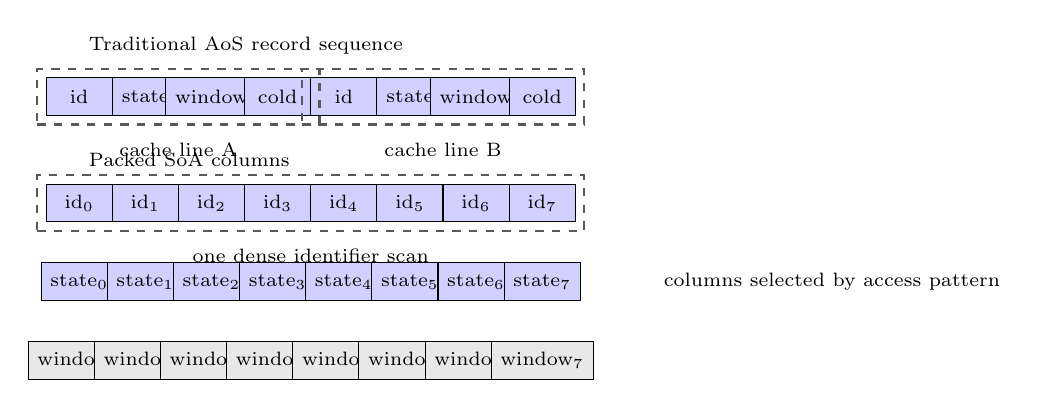
\begin{tikzpicture}[
  font=\scriptsize,
  cell/.style={draw, minimum height=0.48cm, minimum width=0.84cm, align=center},
  cache/.style={draw=black!65, dashed, thick, inner sep=3pt}
]
\node[anchor=west] at (0,2.0) {Traditional AoS record sequence};
\foreach \i/\txt in {0/{id},1/{state},2/{window},3/{cold},4/{id},5/{state},6/{window},7/{cold}} {
  \node[cell,fill=blue!18] (a\i) at (\i*0.84,1.35) {\txt};
}
\node[cache, fit=(a0)(a3)] (ca) {};
\node[cache, fit=(a4)(a7)] (cb) {};
\node[below=0.1cm of ca] {cache line A};
\node[below=0.1cm of cb] {cache line B};
\node[anchor=west] at (0,0.55) {Packed SoA columns};
\foreach \i/\txt in {0/{id$_0$},1/{id$_1$},2/{id$_2$},3/{id$_3$},4/{id$_4$},5/{id$_5$},6/{id$_6$},7/{id$_7$}} {
  \node[cell,fill=blue!18] (s\i) at (\i*0.84,0) {\txt};
}
\node[cache, fit=(s0)(s7)] (cs) {};
\node[below=0.1cm of cs] {one dense identifier scan};
\foreach \i/\txt in {0/{state$_0$},1/{state$_1$},2/{state$_2$},3/{state$_3$},4/{state$_4$},5/{state$_5$},6/{state$_6$},7/{state$_7$}} {
  \node[cell,fill=blue!18] at (\i*0.84,-1.0) {\txt};
}
\foreach \i/\txt in {0/{window$_0$},1/{window$_1$},2/{window$_2$},3/{window$_3$},4/{window$_4$},5/{window$_5$},6/{window$_6$},7/{window$_7$}} {
  \node[cell,fill=gray!18] at (\i*0.84,-2.0) {\txt};
}
\node[anchor=west] at (7.3,-1.0) {columns selected by access pattern};
\end{tikzpicture}
\caption{Conceptual cache line comparison. The shaded AoS cells interleave hot and cold fields, whereas SoA concentrates one field family into a dense scan. The diagram expresses an access pattern hypothesis and is not a processor trace.}
\label{fig:memory}
\end{figure*}

\subsection{SIMD as a bounded transform}

The SIMD module vectorizes byte candidate discovery for HTTP delimiters and field validation. It uses a target dependent lane count, compares a vector against a repeated byte, and falls back to scalar work for candidate verification and the tail. WebSocket masking uses a sixteen byte vector and preserves key position across fragmented buffers by carrying absolute byte position into the scalar tail. These functions do not allocate and do not change input ownership.

\begin{lstlisting}[language=Zig,caption={Source derived form of vectorized WebSocket masking},label={lst:simd}]
pub fn apply_simd(buffer: []u8, masking_key: zslay.MaskingKey,
    position: u64) void {
    if (buffer.len == 0) return;
    var key_bytes: [16]u8 = undefined;
    for (&key_bytes, 0..) |*byte, index| {
        const key_index: usize = @intCast(
            (position +% @as(u64, @intCast(index))) % masking_key.len,
        );
        byte.* = masking_key[key_index];
    }
    const key_vector: Vector = key_bytes;
    var offset: usize = 0;
    while (offset + @sizeOf(Vector) <= buffer.len) :
        (offset += @sizeOf(Vector)) {
        const vector: *align(1) Vector = @ptrCast(buffer[offset..].ptr);
        vector.* = vector.* ^ key_vector;
    }
    apply_scalar(buffer[offset..], masking_key, position +% offset);
}
\end{lstlisting}

The portable vector comparison does not imply identical instructions on all processors. It does imply a vectorizable operation with a scalar path for unsupported targets. The tests compare scalar and SIMD masking, verify position continuity across chunks, and exercise vector and scalar tails. A complete evaluation still requires compiler output inspection and hardware counters.
\section{Multi Protocol Confinement}

Strict Web standards compliance is treated as a sequence of bounded validation and state-transition obligations rather than as an argument for unbounded buffering. The HTTP/1.1 parser validates framing and limits request accumulation under the HTTP semantics of RFC~9112, while the HTTP/2 state machine validates the connection preface, frame sequencing, flow control, and stream lifecycle under RFC~9113; HPACK dynamic-table synchronization follows RFC~7541~\cite{rfc9112,rfc9113,rfc7541}. WebSocket handshakes, masking, fragmentation, close handling, and UTF-8 validation follow RFC~6455, with the pinned Autobahn suite recording 514 \texttt{OK} and three \texttt{INFORMATIONAL} cases out of 517 selected cases~\cite{rfc6455}. Per-Message Deflate follows RFC~7692 while requesting no context takeover and assigning decompression and output to bounded connection-owned regions~\cite{rfc7692}. HTTP/3 and QUIC use the lsquic C boundary with bounded stream, packet, header, and body storage; HTTP/3 framing and QUIC transport/TLS mapping follow RFC~9114, RFC~9000, and RFC~9001, while WebSocket bootstrapping over HTTP/3 validates RFC~9220 metadata without claiming complete live tunnel interoperability~\cite{rfc9114,rfc9000,rfc9001,rfc9220}. WebTransport draft 16 is represented as explicitly bounded settings, session, stream, datagram, capsule, and flow-control state, and unsupported backend capabilities are rejected rather than silently allocated. HTTP QUERY follows RFC~10008 by requiring valid media-type metadata before dispatch~\cite{webtransport,rfc10008}. Finally, BoringSSL supplies TLS~1.3 and ALPN through fixed memory BIO pairs, and disabling TLS~0-RTT keeps replayable early data outside the ordinary admission and storage path~\cite{boringssl,rfc7301,rfc8446}. These boundaries preserve memory safety by making malformed input, capacity exhaustion, and unsupported extensions explicit rejection states.

\subsection{HTTP/1.1}

HTTP/1.1 is confined by a connection owned request accumulator and a strict parser. The parser stores bytes in a fixed request region, validates request line, headers, framing, body size, and expectations, and then shifts only the unconsumed pipelined suffix. The response writer copies validated headers, chunk metadata, and body fragments into a bounded ring. A full ring reports backpressure instead of growing an unbounded list. The router stores route metadata in parallel arrays, seals structural mutation after listening, and gives handlers borrowed request views.

\subsection{HTTP/2 and HPACK}

HTTP/2 introduces multiplexing and state that cannot be represented by one HTTP/1.1 request slot. I use a bounded state machine with a fixed maximum of eight active streams in the TCP integration. The state machine validates the client preface, frame length, stream identifier rules, CONTINUATION sequencing, padding, SETTINGS, flow control, resets, PING, and GOAWAY as required by RFC 9113 \cite{rfc9113}. Each event returns slices borrowing the input frame.

HPACK requires stateful decoding because a header block can reference a connection dynamic table and can be fragmented across frames. The implementation uses a bounded dynamic table, fixed decoded header arrays, caller owned output storage, checked integer decoding, a compile time Huffman tree, and explicit header list limits defined by the HPACK model \cite{rfc7541}. A refused or reset stream still consumes enough compressed input to preserve dynamic table synchronization. The server session maps a stream slot to request storage and asynchronous response state.

The source supports HTTP/2 extended CONNECT WebSocket tunneling and includes tests for protocol validation and accepted tunnel data. The bootstrapping mechanism follows the HTTP/2 WebSocket extension defined by RFC 8441~\cite{rfc8441}. Nevertheless, the one-connection stream slab and connection-owned message region bound the number and shape of concurrent tunnels. If a deployment requires more tunnel state than the configured slab can represent, the server must refuse or close the excess stream, or select an independent HTTP/1.1 connection that can negotiate a conventional upgrade. I describe this as a capacity fallback rather than an in-place protocol conversion.

\subsection{WebSocket and Per Message Deflate}

The WebSocket layer builds on zslay for frame structure and adds handshake validation, fragmentation, close code validation, streaming UTF 8 checking, bounded control frame storage, backpressure, and callback scoped message lifetime under RFC 6455 \cite{rfc6455}. The repository includes a pinned Autobahn runner and source maintained baseline of 517 cases, with 514 classified as \texttt{OK} and three as \texttt{INFORMATIONAL}. I treat this as recorded compliance evidence, not as a performance result generated by this paper.

Per Message Deflate is confined by parsing the extension offer into a small value object and always formatting a response that requests client and server no context takeover under RFC 7692 \cite{rfc7692}. Full window messages use libdeflate, negotiated smaller server windows use preinitialized zlib streams backed by fixed arenas, and incoming output is capped by per connection receive and send scratch. Separate compression input and output regions prevent an outbound callback from overwriting an in progress receive operation.

\subsection{HTTP/3, QUIC, and WebSocket bootstrapping}

The HTTP/3 path uses lsquic through a C interoperation layer and a completion-driven UDP transport. Initialization creates stream, header, and packet pools, together with parallel byte regions for decoded headers, request bodies, response headers, and response bodies. Stream and connection limits derive from compile-time capacity, and QPACK dynamic decoding is disabled by setting its maximum sizes to zero. HTTP/3 framing follows RFC 9114~\cite{rfc9114}, while the underlying transport and TLS integration follow QUIC~\cite{rfc9000,rfc9001}. A new connection, stream, or packet acquires a bounded slot, and exhaustion fails closed or closes the offending stream.

For WebSocket over HTTP/3, the extension module validates RFC 9220 extended CONNECT metadata, including method, protocol, scheme, authority, path, forbidden HTTP/1.1 fields, and WebSocket version 13~\cite{rfc9220}. The validator is zero allocation and retains no header slice after the call. The live lsquic integration supplies HTTP/3 request and response handling and raw datagram capability; the relevant QUIC DATAGRAM extension is specified by RFC 9221~\cite{rfc9221}. Complete RFC 9220 tunnel creation and application WebSocket framing remain outside the live HTTP/3 listener. The current code therefore demonstrates bounded bootstrapping validation, not end-to-end HTTP/3 WebSocket interoperability.

\subsection{WebTransport and HTTP QUERY}

The WebTransport module models draft version 16 with bounded settings, origin and CONNECT checks, generation checked sessions, stream association prefixes, HTTP datagrams, capsules, flow control, and error mapping \cite{webtransport}. It uses fixed session slabs and caller supplied buffers for varint, datagram, and capsule operations. The pinned lsquic capability record exposes raw QUIC datagrams but marks server push and the primitives required by WebTransport draft 16 as unsupported. WebTransport is consequently a bounded protocol and validation surface, not a claim of live interoperability.

HTTP QUERY is live at the router and request validation boundary. The router treats \texttt{QUERY} as a safe body bearing method, supports explicit route registration, and includes it in method negotiation. HTTP/3 and HTTP/2 request paths reject a QUERY request without syntactically valid Content Type before dispatch, while the selected route can impose resource specific media type rules under RFC 10008 \cite{rfc10008}. QUERY reuses ordinary request body storage, routing, response queues, and header validation.

\subsection{TLS and BoringSSL}

The TCP TLS adapter creates a BoringSSL TLS 1.3 server context, installs an ALPN selector that prefers \texttt{h2} and falls back to \texttt{http/1.1}, and attaches a fixed pair of memory BIOs to each connection~\cite{boringssl,rfc7301,rfc8446}. Handshake progress is non-blocking, and plaintext is drained into the same protocol dispatcher used by a non-TLS connection. TLS output is segmented into bounded records before entering the write queue.

The HTTP/3 context advertises only \texttt{h3} and explicitly disables early data. The lsquic engine also sets its delayed 0 RTT packet budget to zero. Rejecting TLS 0 RTT is intentional because replayable application data would require an early data classification and buffering policy that could violate the one request to one storage region correlation. The limitation costs a latency optimization for resumed clients, but preserves a clear memory and replay boundary.


\section{Evaluation Methodology and Profiling}

\subsection{Evidence already present}

The source tree contains unit tests for fixed pool acquisition and release, HTTP delimiter SIMD behavior, scalar and vector WebSocket masking equivalence, no context takeover negotiation, compression buffer separation, HPACK synchronization, HTTP/2 stream and flow control, HTTP/3 header validation, QUERY routing, WebTransport draft state, C ABI boundaries, and TLS ALPN policy. Fuzz targets cover HTTP framing, WebSocket masking, and QUIC packet boundaries. The Autobahn runner verifies the pinned suite against the repository baseline. These checks provide functional evidence for bounded state transitions and protocol rejection behavior, but they do not by themselves establish a cache miss reduction or a tail latency improvement.

\subsection{Repository benchmark and external context}

The repository also defines a reproducible HTTP/1.1 throughput contract~\cite{repo_benchmark}. Table~\ref{tab:repo-benchmark} records the contract rather than an invented result: it fixes the build mode, load generator, concurrency, duration, sample statistic, and relative regression rule. This is useful evidence for repeatability and regression detection. It is not proof that libxev is faster than libuv, because the current repository does not contain a libuv backend or a paired libxev/libuv result set.

\begin{table}[t]
\caption{Repository HTTP throughput contract}
\label{tab:repo-benchmark}
\centering
\begin{tabular}{@{}p{0.30\columnwidth}p{0.57\columnwidth}@{}}
\toprule
Contract field & Frozen setting \\
\midrule
Server and build & \texttt{hello\_world}, Zig \texttt{ReleaseFast} \\
Load generator & \texttt{wrk}; 2 threads, 64 connections, 10 seconds \\
Samples & Three runs; report the median requests per second \\
Endpoint & \texttt{http://127.0.0.1:3000/} \\
Regression rule & Candidate median must be at least 90\% of the baseline median \\
Interpretation & Relative regression guard; not an absolute capacity claim \\
\bottomrule
\end{tabular}
\end{table}

A durable benchmark-data record provides one execution of this contract~\cite{repo_benchmark_record}. The scheduled run used Zig 0.16.0, Nix 2.35.2, two \texttt{wrk} threads, 64 connections, three 10-second samples, and the same source revision for both the recorded baseline and candidate. The candidate median was 177{,}024.21 requests per second versus 173{,}923.95 for the baseline, exceeding the 90\% gate threshold of 156{,}531.56 requests per second. Because the provenance identifies the same source SHA on both sides, this record is best interpreted as a reproducibility and contract-pass record, not as evidence of an implementation improvement. The raw third samples reported p99 latencies of 449~$\mu\text{s}$ for the candidate and 459~$\mu\text{s}$ for the baseline; these are descriptive single-sample observations, not a causal estimate or a confidence interval.

\begin{table}[t]
\caption{Recorded \texttt{http-throughput-v1} result}
\label{tab:repo-result}
\centering
\small
\begin{tabular}{@{}lrr@{}}
\toprule
Build & Median RPS & Three sample RPS values \\
\midrule
Baseline & 173{,}923.95 & 172{,}132.47 / 179{,}453.11 / 173{,}923.95 \\
Candidate & 177{,}024.21 & 175{,}983.07 / 179{,}375.31 / 177{,}024.21 \\
90\% gate & 156{,}531.56 & Passed \\
\bottomrule
\end{tabular}
\end{table}

TechEmpower provides a useful external reference because its benchmark suite covers multiple framework workloads, including plaintext, JSON serialization, database access, and other application tasks~\cite{techempower}. Its Round 23 results are contextual rather than directly comparable: the hardware, client/server topology, framework configuration, test implementation, and measurement round differ from the repository contract. A defensible libxev-versus-libuv claim therefore requires a new paired experiment using the repository contract, plus a clearly identified TechEmpower-compatible implementation if cross-suite comparison is desired.

\subsection{Cache measurement}

I would evaluate the cache hypothesis on a fixed processor and a fixed compiler revision using two server builds with identical protocol limits. The first build would use the current slabs and vector paths. The comparison build would preserve protocol semantics but replace hot slab access with an AoS reference representation and disable SIMD through a compile time switch. The workload would vary concurrent connections, request size, active stream count, WebSocket fragmentation, and output backpressure while keeping request distributions identical.

For each point I would collect instructions, cycles, L1 data cache misses, L2 cache misses, branch misses, allocations, and completed operations. Cachegrind can provide a deterministic first approximation for instruction and simulated cache behavior \cite{cachegrind}, while hardware counters are required to capture the target processor hierarchy. I would report misses per request and misses per byte, not only aggregate counts, because bounded design can change useful work completed at saturation. I would also report the fraction of requests rejected by capacity limits so an apparent locality gain is not purchased by silently doing less work.

\begin{figure}[t]
\centering
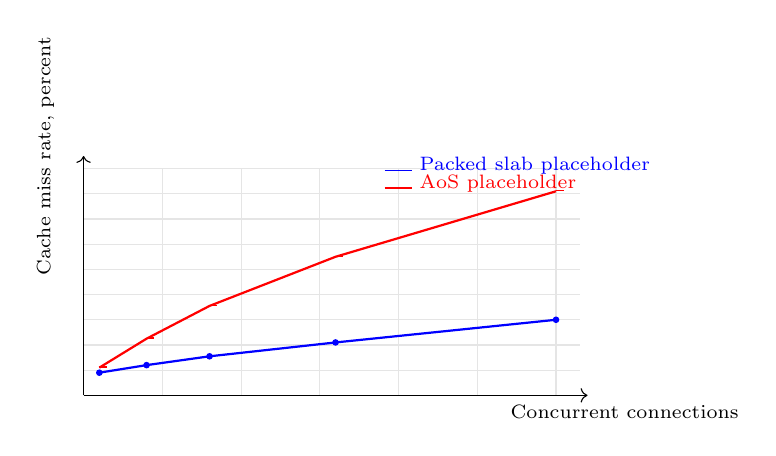
\begin{tikzpicture}
\begin{scope}[x=1cm,y=0.16cm]
  \foreach \x in {1,2,3,4,5,6} {\draw[gray!20] (\x,0) -- (\x,18);}
  \foreach \y in {2,4,6,8,10,12,14,16,18} {\draw[gray!20] (0,\y) -- (6.3,\y);}
  \draw[->] (0,0) -- (6.4,0) node[below right,xshift=-1.1cm] {\scriptsize Concurrent connections};
  \draw[->] (0,0) -- (0,19) node[above,rotate=90,yshift=0.25cm] {\scriptsize Cache miss rate, percent};
  \draw[blue,thick] plot coordinates {(0.2,1.8) (0.8,2.4) (1.6,3.1) (3.2,4.2) (6.0,6.0)};
  \draw[red,thick] plot coordinates {(0.2,2.2) (0.8,4.5) (1.6,7.1) (3.2,11.0) (6.0,16.2)};
  \foreach \x/\y in {0.2/1.8,0.8/2.4,1.6/3.1,3.2/4.2,6.0/6.0} {\fill[blue] (\x,\y) circle (1.2pt);}
  \foreach \x/\y in {0.2/2.2,0.8/4.5,1.6/7.1,3.2/11.0,6.0/16.2} {\fill[red] (\x,\y) rectangle ++(0.10,0.10);}
  \node[anchor=west] at (3.7,18.2) {\scriptsize\textcolor{blue}{\rule{0.35cm}{0.4pt} Packed slab placeholder}};
  \node[anchor=west] at (3.7,16.8) {\scriptsize\textcolor{red}{\rule{0.35cm}{0.4pt} AoS placeholder}};
\end{scope}
\end{tikzpicture}
\caption{Synthetic design placeholder for L1 and L2 cache miss rate versus concurrent connections. The coordinates are not observations and must be replaced by Cachegrind or hardware-counter measurements.}
\label{fig:cache}
\end{figure}

\subsection{Tail latency measurement}

I would measure tail latency with a closed loop client and an open loop overload experiment. The closed loop experiment would estimate service time without queue instability. The open loop experiment would expose admission, output backpressure, and event loop scheduling effects. For the Linux kernel measurement layer, I would use eBPF hooks at socket ingress and egress tracepoints together with uprobes at the libxev completion handoff. Each event would record \texttt{bpf\_ktime\_get\_ns()} and a socket identity into a bounded BPF ring buffer, allowing transport-side timestamps to be compared with user-space completion timestamps without treating a user-space timer as the only clock. This separates kernel queueing and retransmission effects from application processing noise; it does not remove probe overhead or reconstruct protocol request boundaries automatically. The repository currently contains no recorded eBPF trace, so this is the proposed measurement procedure rather than an executed result. I would report median, 95th percentile, 99th percentile, and 99.9th percentile latency, along with queue depth and capacity rejection rate~\cite{ebpf}.

The primary comparison would hold protocol mix constant while changing only memory layout and SIMD configuration. A secondary comparison would vary TLS, compression, HPACK dynamic table activity, and QUIC packet loss separately. A lower tail for plain HTTP/1.1 would not prove that the same architectural mechanism controls compressed WebSocket or multiplexed HTTP/2 traffic.

\begin{figure}[t]
\centering
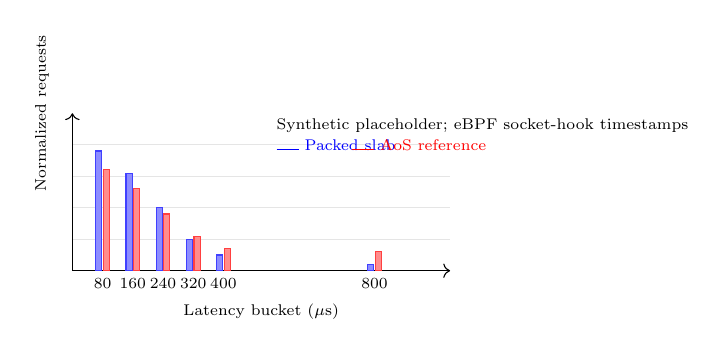
\begin{tikzpicture}[scale=0.8,transform shape]
\begin{scope}[x=0.006cm,y=5cm]
  \draw[gray!20] (0,0.1) -- (1000,0.1);
  \draw[gray!20] (0,0.2) -- (1000,0.2);
  \draw[gray!20] (0,0.3) -- (1000,0.3);
  \draw[gray!20] (0,0.4) -- (1000,0.4);
  \draw[->] (0,0) -- (1000,0);
  \node[below] at (500,-0.08) {\scriptsize Latency bucket ($\mu$s)};
  \draw[->] (0,0) -- (0,0.5) node[above,rotate=90,yshift=0.25cm] {\scriptsize Normalized requests};
  \foreach \x/\label in {80/80,160/160,240/240,320/320,400/400,800/800} {
    \node[below] at (\x,0) {\scriptsize \label};
  }
  \foreach \x/\value in {80/0.38,160/0.31,240/0.20,320/0.10,400/0.05,800/0.02} {
    \pgfmathsetmacro{\leftbar}{\x-18}
    \pgfmathsetmacro{\rightbar}{\x-2}
    \draw[fill=blue!45,draw=blue!75] (\leftbar,0) rectangle (\rightbar,\value);
  }
  \foreach \x/\value in {80/0.32,160/0.26,240/0.18,320/0.11,400/0.07,800/0.06} {
    \pgfmathsetmacro{\leftbar}{\x+2}
    \pgfmathsetmacro{\rightbar}{\x+18}
    \draw[fill=red!45,draw=red!75] (\leftbar,0) rectangle (\rightbar,\value);
  }
  \node[anchor=west,align=left] at (520,0.46) {\scriptsize Synthetic placeholder;\ eBPF socket-hook timestamps};
  \node[anchor=west] at (520,0.40) {\scriptsize\textcolor{blue}{\rule{0.35cm}{0.4pt} Packed slab}};
  \node[anchor=west] at (720,0.40) {\scriptsize\textcolor{red}{\rule{0.35cm}{0.4pt} AoS reference}};
\end{scope}
\end{tikzpicture}
\caption{Tail Latency (99th percentile) Distribution. Synthetic placeholder; values are not measurements.}
\label{fig:tail}
\end{figure}

\subsection{Reproducibility and validity}

I would publish the compiler version, target triple, optimization mode, CPU model, kernel version, NIC configuration, connection limits, route table, protocol mix, random seed, and complete raw trace summaries. I would run the unit, fuzz smoke, C ABI, HTTP/1.1 compliance, and Autobahn gates before each performance comparison. I would repeat each steady state point after warmup and report confidence intervals or quantile bootstrap intervals. I would also test capacity exhaustion, because a bounded server can appear fast when its admission policy rejects requests that would otherwise populate the tail.

The primary threats to validity are hardware dependence, measurement perturbation from tracing, optional library behavior, and the difference between repository baselines and a newly executed test run. Cachegrind is a simulation, not a substitute for hardware counters. eBPF timestamps reveal event boundaries but can perturb scheduling if probes are too broad. I would therefore treat Figures~\ref{fig:cache} and~\ref{fig:tail} as experiment templates, not as results.
\section{Limitations and Architectural Trade offs}

The first limitation is capacity. Fixed connection, stream, packet, header, body, compression, and write regions make memory usage predictable, but a legitimate burst can reach a configured ceiling. The correct response is admission control, backpressure, or a larger preallocated configuration, not an implicit heap allocation. This trade off is suitable for services that prefer bounded failure modes, but it is less convenient for workloads with unbounded message sizes or highly dynamic per tenant state.

The second limitation is indexing. The O(1) freelist does not make every state lookup O(1), and the HTTP/2 stream slab currently uses a bounded scan for stream identifiers. At the default eight stream capacity, the scan has a small fixed upper bound. At a larger capacity, the same policy could become a bottleneck, and adding a hash index would consume additional memory and complicate lifetime synchronization. The design chooses predictable contiguous state over a general purpose map.

The third limitation concerns protocol feature completeness. HTTP/2 extended CONNECT is validated and tested in the live TCP server, yet each connection still carries a bounded stream slab and connection owned message storage. Excess concurrent tunnels must be refused, closed, or handled on a separately negotiated HTTP/1.1 connection. The HTTP/3 extension module validates RFC 9220 metadata, but the current lsquic capability record does not connect complete WebSocket tunnel creation to the live HTTP/3 listener. WebTransport draft 16 is implemented as bounded protocol state and validation helpers, while the repository does not claim live backend interoperability. I therefore avoid describing either helper surface as a production transport feature.

The fourth limitation is compression. No context takeover reduces history retention and makes the memory budget auditable, but it can reduce compression ratio and increase CPU work for repeated messages. Smaller negotiated windows further constrain history and may change throughput for compressible traffic. Allowing arbitrary context reuse would improve some ratios while creating a longer lived state dependency and a larger attack surface. The current policy selects boundedness and isolation.

The fifth limitation is cryptographic startup behavior. BoringSSL TLS 1.3 is integrated through fixed BIO pairs and ALPN, but the QUIC context deliberately rejects TLS 0 RTT. This preserves replay safety and prevents early application data from bypassing ordinary storage admission. The cost is that resumed clients cannot obtain the latency benefit of early data. Any future support would require a per request early data state, replay policy, and storage reservation protocol absent from the current live path.

Finally, cache locality is not monotonic with packing. A very large connection record can evict unrelated hot state, and a dense column can be less useful if a loop always needs several fields together. The repository partly addresses this by separating parallel arrays and reserving cold state alongside hot connection state only where lifetime coupling is strong. The proposed profiler comparison is necessary to decide whether a field belongs in an SoA column, an AoS record, or a separate cold region. Data oriented design is a measured execution technique, not a universal storage rule.

\section{Conclusion}

I analyzed \ensuremath{\mu}WebZockets as a bounded asynchronous protocol system whose principal architectural decision is to make memory capacity explicit at the same level as protocol state. The connection slab, O(1) freelists, HTTP/2 stream SoA, HPACK storage, QUIC pools, caller owned views, SIMD byte transforms, bounded compression regions, and fixed TLS BIOs form one ownership graph. That graph explains why the implementation can avoid steady state general purpose allocation across the principal TCP and QUIC data paths.

The protocol adaptations show that zero allocation is not a single parser trick. HTTP/1.1 requires bounded accumulation and ring output. HTTP/2 requires dynamic table synchronization and stream confinement. WebSocket requires message lifetime discipline, vector masking, and no context takeover compression. HTTP/3 and QUIC require C callback pools and parallel payload regions. WebTransport requires explicit draft state but remains helper only in the current backend. HTTP QUERY reuses existing body and routing limits. BoringSSL requires bounded BIO and record staging, while rejecting 0 RTT preserves the admission boundary.

The current evidence supports a cache locality and high concurrency tail latency hypothesis, not a universal superiority claim. The repository records extensive functional tests and a 514 of 517 successful Autobahn baseline, but the cache and latency figures in this paper are intentionally synthetic placeholders. I would consider the architectural thesis established only after the proposed controlled comparison reports hardware counters, allocation counts, capacity rejection rates, and tail distributions across equivalent protocol workloads.
\bibliographystyle{IEEEtran}
\bibliography{ref}
\end{document}
